\documentclass[12pt,]{tufte-handout}

% ams
\usepackage{amssymb,amsmath}

\usepackage{ifxetex,ifluatex}
\usepackage{fixltx2e} % provides \textsubscript
\ifnum 0\ifxetex 1\fi\ifluatex 1\fi=0 % if pdftex
  \usepackage[T1]{fontenc}
  \usepackage[utf8]{inputenc}
\else % if luatex or xelatex
  \makeatletter
  \@ifpackageloaded{fontspec}{}{\usepackage{fontspec}}
  \makeatother
  \defaultfontfeatures{Ligatures=TeX,Scale=MatchLowercase}
  \makeatletter
  \@ifpackageloaded{soul}{
     \renewcommand\allcapsspacing[1]{{\addfontfeature{LetterSpace=15}#1}}
     \renewcommand\smallcapsspacing[1]{{\addfontfeature{LetterSpace=10}#1}}
   }{}
  \makeatother

\fi

% graphix
\usepackage{graphicx}
\setkeys{Gin}{width=\linewidth,totalheight=\textheight,keepaspectratio}

% booktabs
\usepackage{booktabs}

% url
\usepackage{url}

% hyperref
\usepackage{hyperref}

% units.
\usepackage{units}


\setcounter{secnumdepth}{-1}

% citations


% pandoc syntax highlighting

% table with pandoc

% multiplecol
\usepackage{multicol}

% strikeout
\usepackage[normalem]{ulem}

% morefloats
\usepackage{morefloats}


% tightlist macro required by pandoc >= 1.14
\providecommand{\tightlist}{%
  \setlength{\itemsep}{0pt}\setlength{\parskip}{0pt}}

% title / author / date
\title{Tufte Handout}
\author{Your Name}
\date{2024-07-16}


\begin{document}

\maketitle




\section{Executive Summary}\label{executive-summary}

\section{Purpose}\label{purpose}

An estimated 450,000 to 470,000 individuals in TN are being denied their
right to vote due to incarceration, disproportionately affecting African
American voters. Our purpose is to determine how many individuals are
disenfranchised, specifically in each county in the state of Tennessee.

\subsection{Methods}\label{methods}

Analysis and Report In order to make our findings most useful for
policymakers and legislators, we used R Markdown to incorporate our
findings into the final deliverable for Dr.~Sekou Franklin, a written
report. Our analysis consisted of mapping data using choropleths to
visualize trends as well as charting findings in tables. The written
report is the most suitable format for presentation to legislators and
policy makers.

\subsubsection{Data Acquisition}\label{data-acquisition}

There is no standardized tracking system in place that houses
county-level data on the number of disenfranchised individuals who are
eligible to restore their voting rights. To circumvent this roadblock,
we obtained an estimate of the number of people impacted by county and
how it affects local elections. Then, we performed web scraping, data
cleaning, and data exploration with visualizations to illustrate our
findings.

\subsubsection{Dataset Merging}\label{dataset-merging}

We merged relevant datasets to create original ones, enabling us to
approach our question from a fresh perspective beyond providing a single
numerical answer. We merged the voter turnout data with the census data
to analyze what demographics might influence voter turnout by county.

\subsubsection{Analysis}\label{analysis}

In order to make our findings most useful for policymakers and
legislators, we used R Markdown to incorporate our findings into the
final deliverable for Dr.~Sekou Franklin, a written report. Our analysis
consisted of mapping data using choropleths to visualize trends as well
as charting findings in tables. The written report is the most suitable
format for presentation to legislators and policy makers.

\subsection{Key Findings}\label{key-findings}

We built the Tennessee county map (see Figure 1) to illustrate the
patterns in the voter turnout and compare with the demographics of each
county. Then, we charted the incarceration rate by felony type (see
Figure 2) to get an estimate of the ratio of individuals who have the
possibility of restoring their rights upon release versus those who do
not. One of the most immediately apparent observations is that most
people convicted of a felony are not due to violent crimes and thus
could have their rights restored were it not for legal financial
obligations (LFOs).

Figure 1. 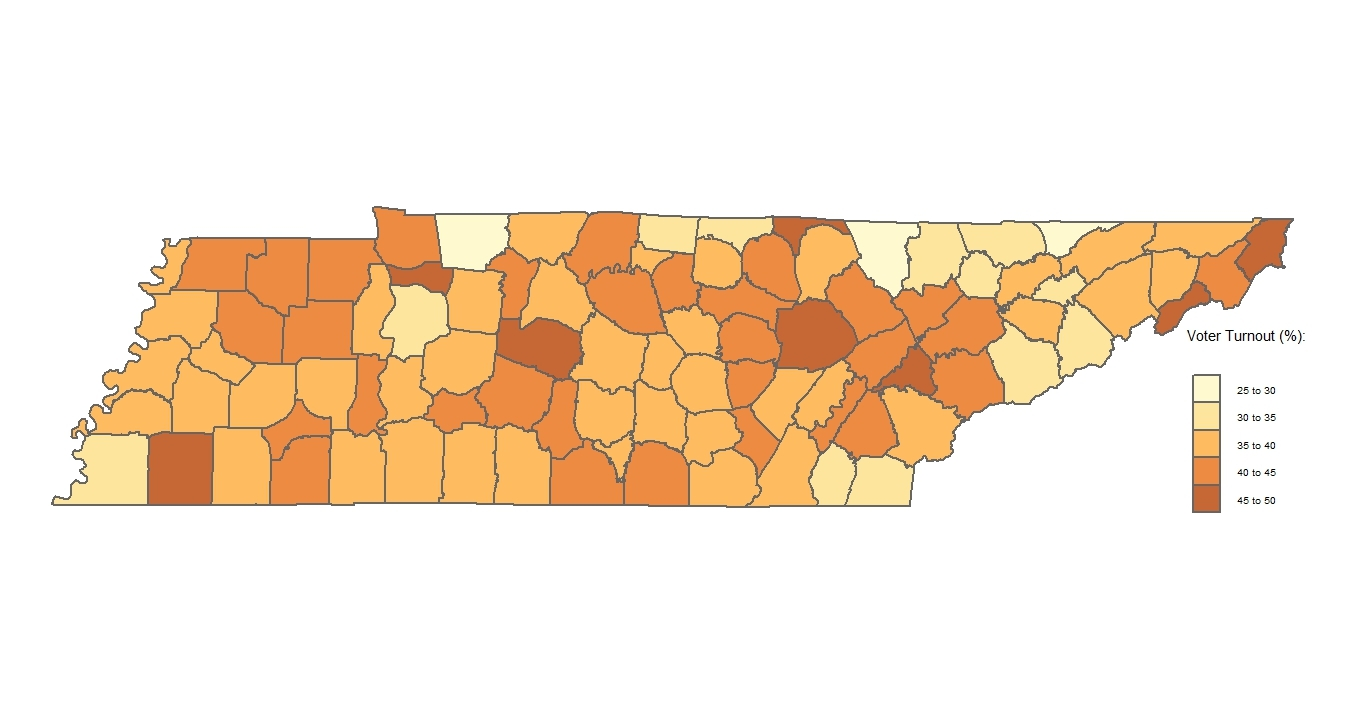
\includegraphics{Rplot05.jpeg}

Figure 2.

\begin{figure}
\centering
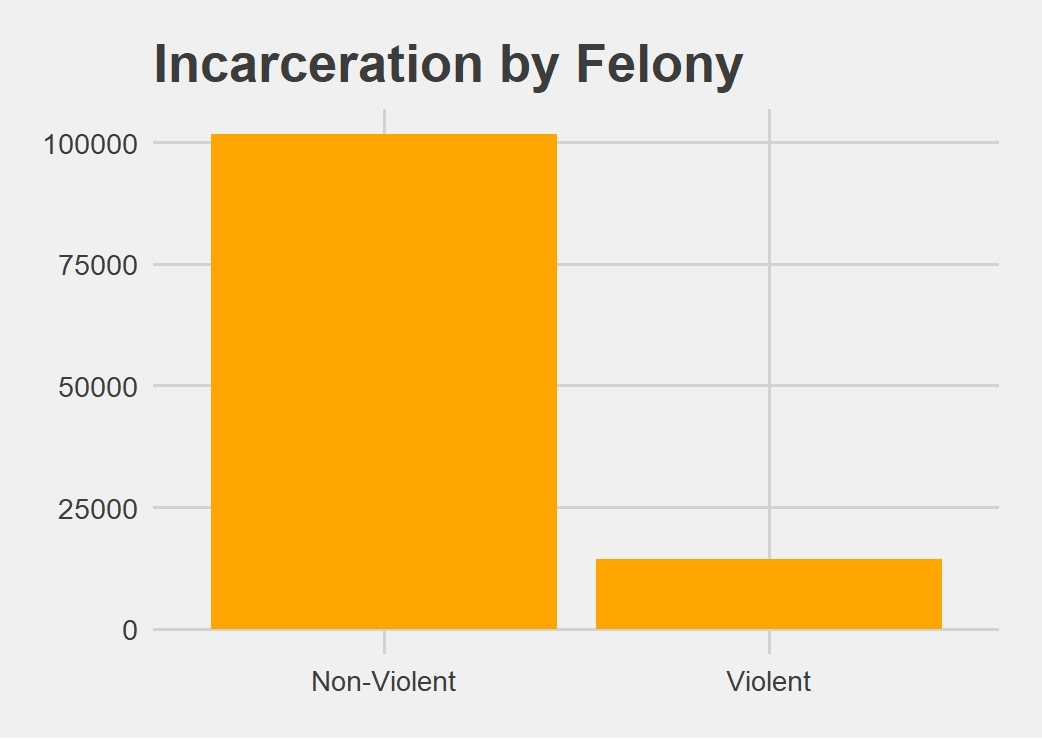
\includegraphics[width=0.5\textwidth,height=\textheight]{plot plotototroto.jpeg}
\caption{Incarceration By Felony}
\end{figure}

Figure 3.

\begin{figure}
\centering
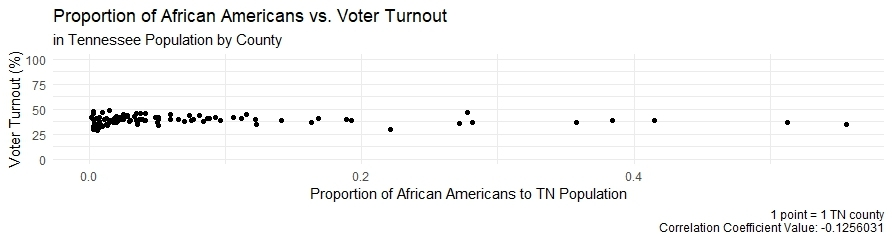
\includegraphics[width=4\textwidth,height=\textheight]{prop_aa_pop_vt.jpeg}
\caption{Measuring Correlation Coefficient Value}
\end{figure}

This plot shows that in the state of Tennessee, voter turnout by county
varies from 29.3\% to 48.4\% and does not depend in a statistically
significant way on the African American population or income level. On
the other hand, it is important to note that very few counties have an
African American population over \textasciitilde20\%. Although the
African American Tennesseans make up only 17\% of the state's
population, 40\% of them are state prisoners. Additionally, the bar
chart above visualizes that there are currently around 100,000 people
incarcerated for felonies in the state of TN; the rest of the
disenfranchised population have already served their time and have been
released.

\begin{figure}
\centering
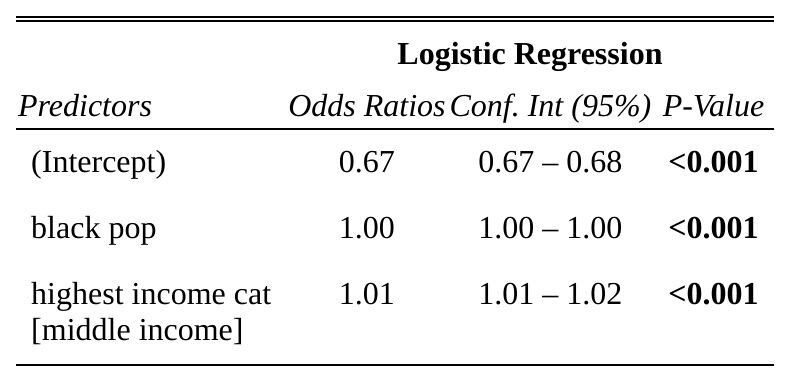
\includegraphics[width=0.7\textwidth,height=\textheight]{tfdr2 (1).jpg}
\caption{Logistic Regression}
\end{figure}

This chart comepares\ldots{}

\section{Conclusion}\label{conclusion}

Although the data on disenfranchisement is bare, the impact of our
research is substantial. Through the research process, we found that
voter disenfranchisement is not discussed enough nor tracked enough. The
findings will aid in raising awareness of the issue and the importance
of thorough data collection. Additionally, our study highlights the
disproportionate impact of disfranchisement on minority communities due
to lack of representation by elected officials.

\section{Implications}\label{implications}

What we've found is\ldots.?



\end{document}
